\chapter{Model Architectures}
\label{sec:models}

This chapter presents the PIVOT architecture and seven dynamics models of increasing expressiveness, all trained on $\mathcal{D}_{\text{train}}$. Section~\ref{sec:overview} describes the overall pipeline. Section~\ref{sec:visual-context} defines the visual context representation $\xi^{(i)}$. Section~\ref{sec:param-generator} details the parameter generator $\psi$. Section~\ref{sec:dynamics-models} specifies each dynamics model $\hat{f}$. Section~\ref{sec:efficient-rollout} explains the rollout design that enables real-time control. Table~\ref{tab:models} summarizes the model characteristics, and Table~\ref{tab:param-counts} reports parameter counts.

%--------------------------------------------------
\section{Overview}
\label{sec:overview}

All five learned models (LST, LTVL, MLP, LSTM, TCN) share a common two-stage architecture that separates parameter estimation from dynamics rollout:

\begin{enumerate}
  \item \textbf{Parameter estimation.} A shared parameter network $\psi$ maps context features $\xi^{(i)}$ to a compact parameter vector $\phi^{(i)}$. This mapping executes once per control cycle.
  \item \textbf{Dynamics rollout.} The dynamics model $\hat{f}$ consumes $\phi^{(i)}$ and rolls out a predicted trajectory over the $H$-step prediction horizon. The same $\phi^{(i)}$ is reused at every step within the horizon.
\end{enumerate}

The parameter network and dynamics model are trained jointly: the optimizer backpropagates a yaw-normalized L1 loss through the integrator and dynamics equations into the parameter network weights, which are the only trainable variables. The dynamics computation is fully differentiable in JAX, and optimization employs Adam with a learning rate of $10^{-3}$.

The models differ in the dimensionality of $\phi^{(i)}$ (Table~\ref{tab:param-counts}). The LST model requires only 17 outputs (9 physical parameters and 8 residual corrections) because the nonlinear bicycle dynamics handle the bulk of the prediction. The data-driven models require the parameter network to output the entire weight set of the dynamics model: 838 values for the MLP, 821 for the TCN, and 19,141 for the LSTM. Although these dynamics models are small by deep learning standards, the parameter network's output layer scales with the target dimensionality (e.g., $\approx$4.9M parameters for the LSTM output layer alone, 5.7$\times$ the shared backbone), amplifying the risk of overfitting on limited real-world data.

Two fixed-parameter baselines (DST, DTVL) bypass the parameter network entirely: their parameters are identified offline via system identification on $\mathcal{D}_{\text{train}}$, and remain constant during deployment. This controlled setup isolates the effect of model architecture on prediction accuracy and control performance.

%--------------------------------------------------
\section{Visual Context Representation}
\label{sec:visual-context}

The context feature vector $\xi^{(i)}$ encodes both visual and proprioceptive information about the current operating condition. It comprises two components.

\paragraph{Semantic visual features.}
A frozen DINOv2 ViT-S/14 backbone~\cite{oquab2024dinov2} extracts a 384-dimensional CLS token from each onboard camera image ($854 \times 480$ pixels, 30\,Hz). The image is resized to 256 pixels on the shorter side, center-cropped to $224 \times 224$, and normalized with ImageNet statistics before being passed through the network. The resulting feature vector is L2-normalized to unit norm. DINOv2 is selected for its ability to produce semantically rich representations without task-specific fine-tuning: the frozen backbone captures terrain texture, surface type, and scene geometry in a compact embedding that generalizes across visual conditions. Figure~\ref{fig:dino-features} visualizes the patch-level DINOv2 features for two scenes from the test track, illustrating how the representation distinguishes terrain regions (grass, pavement, buildings) without any task-specific supervision.

\begin{figure}[t]
  \centering
  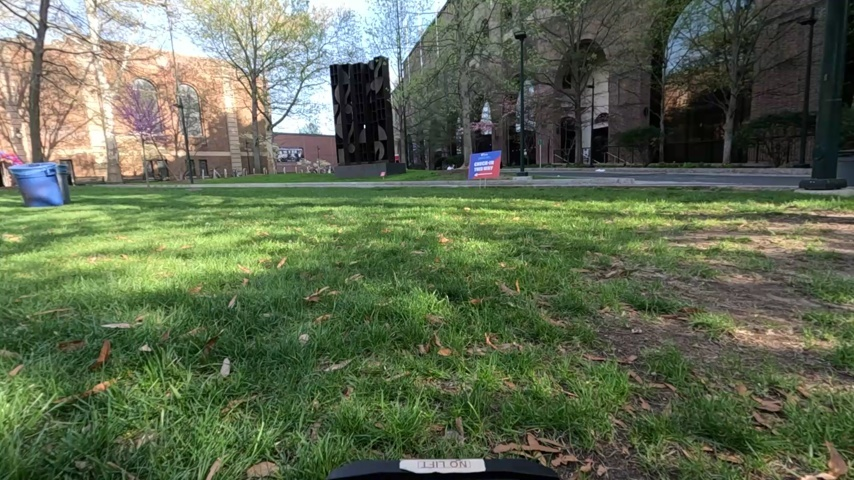
\includegraphics[height=2.6cm]{img/dino_feature/image_1776202324420642048.jpg}\kern1pt
  
\includegraphics[height=2.6cm]{img/dino_feature/image_1776202324420642048_feature.png}\hspace{0.8em}
  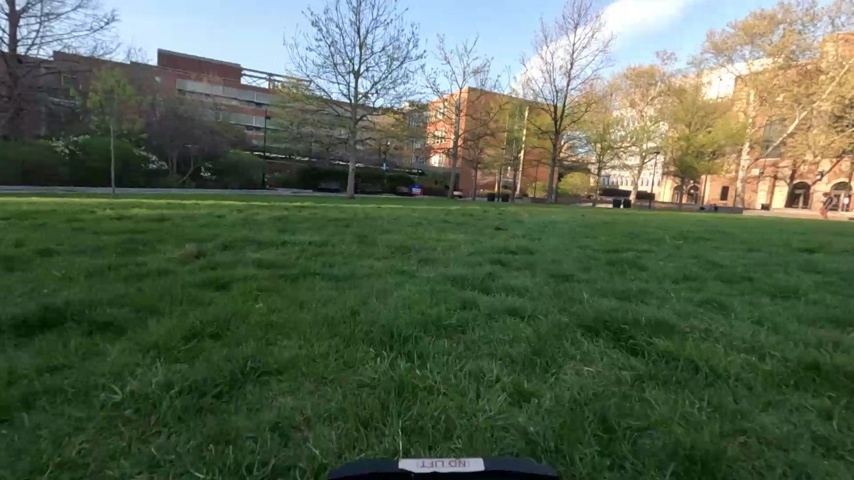
\includegraphics[height=2.6cm]{img/dino_feature/image_1776206037414451712.jpg}\kern1pt
  
\includegraphics[height=2.6cm]{img/dino_feature/image_1776206037414451712_feature.png}

  \caption{Onboard camera images (left of each pair) and corresponding DINOv2 patch-level feature visualizations (right of each pair) from two locations on the test track. Colors in the feature maps encode the NCUT spectral eigenvectors of the patch token embeddings, projected to RGB via UMAP. Semantically distinct regions (grass, pavement, buildings, sky) produce distinct feature clusters without task-specific fine-tuning}
  \label{fig:dino-features}
\end{figure}

\paragraph{State context.}
An 8-dimensional proprioceptive vector captures the vehicle's instantaneous kinematic state: body-frame velocities $(v_x, v_y, v_z)$, yaw rate $\dot{\psi}$, pitch $\theta$ and pitch rate $\dot{\theta}$, and roll $\varphi$ and roll rate $\dot{\varphi}$. These quantities are measured by the onboard IMU and GNSS system at 100\,Hz. State context provides the parameter network with information about the current dynamic regime (e.g., high-slip cornering versus straight-line driving) that is not directly visible in the camera image.

The two components are concatenated to form the context feature vector:
\begin{equation}
  \xi^{(i)} = \bigl[\,\underbrace{z_{\text{DINOv2}}}_{\text{384-dim}},\;\; \underbrace{s_{\text{ctx}}}_{\text{8-dim}}\,\bigr] \in \mathbb{R}^{392}.
  \label{eq:context-features}
\end{equation}
The DINOv2 backbone is frozen during training; only the parameter network $\psi$ is updated.

%--------------------------------------------------
\section{Parameter Generator}
\label{sec:param-generator}

The parameter generator $\psi$ maps the context feature vector $\xi^{(i)}$ to a dynamics parameter vector $\phi^{(i)} \in \mathbb{R}^{d_\phi}$, where $d_\phi$ depends on the downstream dynamics model.

\paragraph{Architecture.}
The generator is a multi-layer perceptron with PReLU activations and batch normalization between layers. It comprises two components: a shared backbone and a model-specific output stage. The backbone ($\approx$858K parameters) is identical across all five learned models, ensuring that architectural differences in downstream dynamics are not confounded by differences in feature extraction capacity.

\paragraph{Multi-head output.}
The output stage employs multiple parameter heads, each producing a candidate parameter vector. A discriminator head outputs softmax-weighted selection probabilities over the candidates. The final parameter vector is the probability-weighted average of all heads:
\begin{equation}
  \phi^{(i)} = \sum_{m=1}^{M} \alpha_m \cdot \phi^{(i)}_m, \qquad \alpha_m = \frac{\exp(d_m)}{\sum_{m'}\exp(d_{m'})},
\end{equation}
where $\phi^{(i)}_m$ denotes the $m$-th head output and $d_m$ the corresponding discriminator logit. This mixture-of-experts structure allows the network to represent multimodal parameter distributions (e.g., distinct terrain regimes) without committing to a single prediction.

\paragraph{Output scaling.}
Each predicted parameter is passed through a scaled tanh function that maps the raw network output into a physically meaningful range $[\phi_{\min}, \phi_{\max}]$:
\begin{equation}
  \phi_j = \frac{\phi_{\max,j} - \phi_{\min,j}}{2}\,\big(\tanh(x_j) + 1\big) + \phi_{\min,j}.
\end{equation}
The bounds are set based on physical plausibility (e.g., mass $> 0$, friction coefficient $\in [0, 2]$), preventing the optimizer from exploring unphysical parameter regions during training.

%--------------------------------------------------
\section{Dynamics Models}
\label{sec:dynamics-models}

Seven dynamics models are evaluated, grouped into three categories. All models predict continuous-time state derivatives that are discretized via numerical integration (Section~\ref{sec:efficient-rollout}), except as noted.

%--------------------------------------------------
\subsection{Fixed-Parameter Physics Models}
\label{sec:fixed}

These models employ conventional offline system identification with no learned components, serving as baselines.

\subsubsection{Default Single-Track Model (DST)}
\label{sec:dst}

The default single-track model is a nonlinear bicycle model with a 7-dimensional state
\begin{equation}
  s = [x,\, y,\, \delta,\, v,\, \psi,\, \dot{\psi},\, \beta]^\top,
\end{equation}
representing position $(x, y)$, steering angle $\delta$, longitudinal velocity $v$, heading $\psi$, yaw rate $\dot{\psi}$, and sideslip angle $\beta$. The two control inputs are
\begin{equation}
  a = [\dot{\delta},\, a_{\text{long}}]^\top,
\end{equation}
where $\dot{\delta}$ denotes the steering rate and $a_{\text{long}}$ the longitudinal acceleration.

The model employs a velocity-dependent switching mechanism. At low speeds ($|v| < 1.5$\,m/s), a kinematic formulation governs the dynamics. At higher speeds, a dynamic formulation with nonlinear tire force modeling becomes active. The continuous-time dynamics are discretized via fourth-order Runge--Kutta (RK4) integration with time step $\Delta t$.

The 14 physical parameters, including mass ($m = 3.74$\,kg), yaw inertia ($I_z = 0.047$\,kg$\cdot$m$^2$), front and rear cornering stiffness ($C_{Sf} = 4.72$, $C_{Sr} = 5.46$), and tire-road friction coefficient ($\mu = 1.05$), are identified offline via system identification. State constraints enforce steering limits of $\pm 0.42$\,rad, velocity bounds of $[-5, 20]$\,m/s, and steering rate limits of $\pm 3.2$\,rad/s.

\subsubsection{Default Time-Varying Linear Model (DTVL)}
\label{sec:dtvl}

The default time-varying linear model adopts a 5-dimensional state $s = [x,\, y,\, \delta,\, v,\, \psi]^\top$ with the same two control inputs. The dynamics take the form
\begin{equation}
  \dot{s} = A \begin{bmatrix} s \\ a \end{bmatrix} + B,
  \label{eq:tvl}
\end{equation}
where $A \in \mathbb{R}^{5 \times 7}$ and $B \in \mathbb{R}^{5}$ are fixed matrices identified offline. This model captures dynamics only in the vicinity of the nominal operating point around which linearization is performed, limiting its efficacy under aggressive maneuvers.

%--------------------------------------------------
\subsection{Physics-Informed Learned Models (PIVOT)}
\label{sec:physics-learned}

The two proposed PIVOT models retain known physics structure while adapting model parameters as functions of the context features $\xi^{(i)}$. By preserving established dynamics equations as an inductive bias, these architectures target improved sample efficiency and generalization compared to purely data-driven alternatives.

\subsubsection{Learned Single-Track Model (LST)}
\label{sec:lst}

The learned single-track model shares the same nonlinear bicycle dynamics and velocity-dependent switching mechanism as the DST model (Section~\ref{sec:dst}), but augments four dynamics channels with learnable corrections. Specifically, the steering rate ($\dot{\delta}$), longitudinal acceleration ($\dot{v}$), yaw acceleration ($\ddot{\psi}$), and sideslip rate ($\dot{\beta}$) channels are each modified as
\begin{equation}
  \dot{s}_j = f_{\text{physics},j}(s, a) \cdot \alpha_j + \beta_j,
  \label{eq:lst-augment}
\end{equation}
where $f_{\text{physics},j}$ denotes the original physics-based computation for the $j$-th channel, and $\alpha_j$, $\beta_j$ are learnable multiplicative gains and additive biases, respectively.

The parameter network predicts a total of 17 values from the context features:
\begin{equation}
  [\underbrace{m, I_z, l_f, l_r, h, C_{Sf}, C_{Sr}, \mu, L}_{\text{9 physical}},\;\; \underbrace{\alpha_1, \beta_1, \ldots, \alpha_4, \beta_4}_{\text{8 augmentation}}] = \psi_{\text{LST}}(\xi^{(i)}).
\end{equation}
The 9 physical parameters (mass, yaw inertia, front and rear axle distances, center-of-gravity height, front and rear cornering stiffness, friction coefficient, and vehicle length) replace the fixed values in the bicycle model equations, enabling the network to adapt tire and inertial properties to the current terrain. The 8 augmentation parameters provide residual corrections beyond what the physical parameter space can express. Gains are initialized to $\alpha_j = 1$ and biases to $\beta_j = 0$, ensuring that the model recovers the default single-track dynamics at initialization. The augmented dynamics are integrated via RK4, and the network is trained end-to-end by backpropagating through the integrator.

The LST model thus performs two complementary functions: (1) inferring terrain-dependent physical properties (e.g., reducing $\mu$ on wet grass, adjusting $C_{Sf}$ and $C_{Sr}$ for tire wear), and (2) compensating for structural model mismatch via residual corrections. The nonlinear bicycle dynamics handle the bulk of the prediction, and the network provides only calibration and residual compensation.

\subsubsection{Learned Time-Varying Linear Model (LTVL)}
\label{sec:ltvl}

The learned time-varying linear model extends the DTVL model (Section~\ref{sec:dtvl}) by replacing the fixed matrices with context-dependent ones predicted by the parameter network:
\begin{equation}
  \dot{s} = A(\xi^{(i)})\begin{bmatrix} s \\ a \end{bmatrix} + B(\xi^{(i)}),
  \label{eq:ltvl}
\end{equation}
where
\begin{equation}
  [A(\xi^{(i)}),\, B(\xi^{(i)})] = \psi_{\text{LTVL}}(\xi^{(i)}).
\end{equation}
The parameter network outputs the 40 values comprising the flattened matrix $A \in \mathbb{R}^{5 \times 7}$ and bias $B \in \mathbb{R}^{5}$. The predicted dynamics are integrated via RK4.

In contrast to the DTVL model, this formulation represents globally nonlinear dynamics through context-dependent linearization while preserving linear structure at each operating point, offering a trade-off between the interpretability of linear models and the expressiveness of nonlinear ones.

%--------------------------------------------------
\subsection{Purely Data-Driven Models}
\label{sec:data-driven}

These models learn dynamics entirely from data without explicit physics structure. All three adopt the same 5-dimensional state $s = [x,\, y,\, \delta,\, v,\, \psi]^\top$ and two control inputs as the DTVL model, and predict state derivatives $\dot{s}$ with a time step of $\Delta t = 0.05$\,s. In the PIVOT framework, the parameter network generates the entire weight set of each dynamics model, effectively functioning as a hypernetwork.

\subsubsection{Multi-Layer Perceptron (MLP)}
\label{sec:mlp}

A feedforward network with a single hidden layer of 64 units and tanh activations maps the concatenated state-action vector to state derivatives:
\begin{equation}
  \dot{s} = W_2 \tanh\!\big(\alpha\,(W_1 [s^\top, a^\top]^\top + b_1)\big) + b_2,
\end{equation}
where $\alpha$ is a learnable activation scale. The parameter network outputs all 838 weights ($W_1, b_1, W_2, b_2, \alpha$). As a memoryless model, the MLP captures instantaneous nonlinear mappings but cannot exploit temporal structure in the data.

\subsubsection{Long Short-Term Memory Network (LSTM)}
\label{sec:lstm}

The LSTM employs a single-layer cell with 64 hidden units and four standard gates (input, forget, cell candidate, and output), allowing the network to selectively retain or discard information across timesteps. The heading angle $\psi$ is represented as $[\sin\psi,\, \cos\psi]$ to avoid the discontinuity at $\pm\pi$, yielding the input vector $[\tilde{s}_t^\top, a_t^\top]^\top \in \mathbb{R}^{8}$ with $\tilde{s}_t = [x,\, y,\, \delta,\, v,\, \sin\psi,\, \cos\psi]^\top$. The LSTM cell processes this input and produces a state update via an output projection:
\begin{equation}
  h_t, c_t = \text{LSTM}(\tilde{s}_t, a_t, h_{t-1}, c_{t-1};\, \phi_{\text{LSTM}}), \qquad \Delta s_t = W_{\text{out}}\, h_t + b_{\text{out}}.
\end{equation}
Euler integration yields the next state as $s_{t+1} = s_t + \Delta s_t$, rather than the RK4 scheme employed by the other models. RK4 evaluates the dynamics function at multiple intermediate points per timestep. For a recurrent model, each intermediate evaluation advances the hidden state, causing the memory to drift from the trajectory it is meant to represent. Euler integration evaluates the LSTM cell exactly once per timestep, preserving a consistent correspondence between hidden state and trajectory history.

During training, a burn-in phase (a sequence of preceding timesteps processed without loss computation) initializes the hidden state before the loss is evaluated. The parameter network outputs all 19,141 weights comprising the gate matrices, output projection, and initial hidden and cell states.

\subsubsection{Temporal Convolutional Network (TCN)}
\label{sec:tcn}

The TCN maintains a sliding buffer of the $K = 4$ most recent state-action pairs. At each timestep, the current pair replaces the oldest entry, and the network processes the buffer through two causal 1D convolutional layers (kernel sizes 4 and 1, with a hidden dimension of 16 and tanh activations) followed by a linear output projection to state derivatives:
\begin{equation}
  \dot{s}_t = W_{\text{out}}\, \text{Conv}_2\!\big(\tanh(\text{Conv}_1(\text{buf}_t))\big) + b_{\text{out}}.
\end{equation}

Unlike the LSTM, the TCN can employ RK4 integration because its buffer remains fixed during the intermediate sub-steps of each timestep: only the final integrated state updates the buffer for the next step. This avoids the hidden-state drift that prevents the LSTM from employing higher-order integrators. The parameter network outputs all 821 weights comprising the convolutional kernels and output projection.

%--------------------------------------------------
\section{Efficient Rollout Design}
\label{sec:efficient-rollout}

Deploying learned dynamics within a sampling-based controller such as MPPI imposes strict computational constraints. At each control cycle, MPPI samples $K$ candidate control sequences and rolls out each through the dynamics model over the $H$-step horizon. A naive implementation that invokes the parameter network at every step of every sample incurs $K \times H$ forward passes.

The two-stage architecture eliminates this bottleneck. The parameter network executes once per control cycle, producing a single parameter vector $\phi^{(i)}$ from the current context features. The dynamics model then rolls out all $K$ candidate trajectories using the same $\phi^{(i)}$. This factorization reduces the parameter network cost from $O(K \cdot H)$ to $O(1)$ per control cycle.

\paragraph{Vectorized rollout.}
The dynamics computation is implemented in JAX, enabling vectorized rollout of all $K$ trajectories in parallel via \texttt{jax.vmap}. Because each trajectory shares the same parameter vector, the rollout reduces to a batched scan over timesteps with no per-sample branching.

\paragraph{Numerical integration.}
Continuous-time state derivatives are discretized via fourth-order Runge--Kutta (RK4) integration for all models except the LSTM, which employs Euler integration to preserve hidden-state consistency (Section~\ref{sec:lstm}). The TCN employs RK4 with its temporal buffer held fixed during sub-steps. A configurable sub-stepping ratio allows finer integration resolution without changing the control timestep.

\paragraph{Computational cost.}
The parameter network ($\approx$858K parameters) adds negligible overhead relative to the rollout computation. For the LST model with $K = 512$ samples and $H = 9$ steps, the complete control cycle (parameter prediction and trajectory rollout) executes within the real-time budget of a 50\,Hz control loop, occupying less than 3\% of the 20\,ms cycle on an NVIDIA RTX A6000. The dominant cost is the dynamics rollout itself, not the parameter network, confirming that the two-stage factorization achieves its design goal.

%--------------------------------------------------
\begin{table}[t]
\centering
\caption{Summary of the seven dynamics models evaluated in this work. LST and LTVL are the proposed PIVOT models; the remaining five serve as baselines. Physics-informed models retain known dynamics equations, while data-driven models learn the full state-derivative mapping from data. Temporal models incorporate past state-action history.}
\label{tab:models}
\small
\begin{tabular}{@{}llcccc@{}}
\toprule
Category & Model & Dim. & Learned & Physics & Temporal \\
\midrule
\multirow{2}{*}{Fixed} & DST & 7 & -- & \checkmark & -- \\
 & DTVL & 5 & -- & \checkmark & -- \\
\midrule
\multirow{2}{*}{PIVOT} & LST & 7 & \checkmark & \checkmark & -- \\
 & LTVL & 5 & \checkmark & \checkmark & -- \\
\midrule
\multirow{3}{*}{Data-Driven} & MLP & 5 & \checkmark & -- & -- \\
 & LSTM & 5 & \checkmark & -- & \checkmark \\
 & TCN & 5 & \checkmark & -- & \checkmark \\
\bottomrule
\end{tabular}
\end{table}

\begin{table}[t]
\centering
\caption{Parameter counts for each learned model. All models share the same 858K-parameter backbone; the output layer scales with the number of predicted dynamics parameters. The LST model requires only 17 outputs, keeping total parameters near the backbone size, while the LSTM requires 19,141 outputs, inflating the total to 5.8M and increasing overfitting risk.}
\label{tab:param-counts}
\small
\begin{tabular}{@{}lrrr@{}}
\toprule
Model & Dynamics Params & Output Layer & Total \\
\midrule
LST & 17 & 4,369 & 862,225 \\
LTVL & 40 & 10,280 & 868,136 \\
MLP & 838 & 215,366 & 1,073,222 \\
TCN & 821 & 210,997 & 1,068,853 \\
LSTM & 19,141 & 4,919,237 & 5,777,093 \\
\bottomrule
\end{tabular}
\end{table}
